\chapter{电磁学}

\newpage
{\bf 这里是一段关于电磁学的介绍.}

\newcommand\resistance{
	\begin{tikzpicture}[baseline = {([yshift = -3.5pt] current bounding box.center)}]
		\draw (0, 0) rectangle (0.6, 0.2);
		\draw (-0.3, 0.1) -- (0, 0.1);
		\draw (0.6, 0.1) -- (0.9, 0.1);
	\end{tikzpicture}
}

\newcommand\ammeter{
	
\begin{tikzpicture}[baseline = {([yshift = -3.5pt] current bounding box.center)}]
		\node (A) [circle, draw, scale = 1, inner sep = 1pt, line width = 0.5pt] at (0, 1){\small A};
	\end{tikzpicture}
} % ~{\Large\textcircled{\small A}}~

\newcommand\voltmeter{
	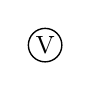
\begin{tikzpicture}[baseline = {([yshift = -3.5pt] current bounding box.center)}]
		\node (V) [circle, draw, scale = 1, inner sep = 1pt, line width = 0.5pt] at (0, 1){\small V};
	\end{tikzpicture}
} % ~{\Large\textcircled{\small V}}~

\newcommand\slidingrheostat{
	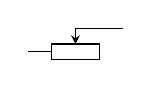
\begin{tikzpicture}[baseline = {([yshift = -3.5pt] current bounding box.center)}]
		\draw (0, 0) rectangle (0.6, 0.2);
		\draw (-0.3, 0.1) -- (0, 0.1);
		\draw [-stealth] (0.3, 0.4) -- (0.3, 0.2);
		\draw [line join = miter] (0.9, 0.4) -- (0.3, 0.4) -- (0.3, 0.3);
	\end{tikzpicture}
}

\section{电荷}

\vspace{10pt}
\begin{itemize}
\item 物体能够吸引轻小物体,就说物体带了电,即物体带了\blue{电荷}(electric charge)。带了电荷的物体叫做\blue{带电体}。
\item 使物体带电叫做\blue{起电}。用摩擦的方式使物体带电叫做\blue{摩擦起电}(electrification by friction)。
\item 自然界\blue{只有}两种电荷。
\item 用丝绸摩擦过的玻璃棒带的电荷叫做\blue{正电荷}(positive charge)。用毛皮摩擦过的橡胶棒带的电荷叫做\blue{负电荷}(negative charge)。
\item \blue{同种}电荷相互\blue{排斥},\blue{异种}电荷相互\blue{吸引}。
\item 电荷的多少叫做\blue{电荷量}(electric quantity),简称\blue{电量}。用 \blue{$\bm Q$} 或 \blue{$\bm q$} 表示。在国际单位制中,电荷量的单位是\blue{库仑}(coulomb),简称\blue{库}。符号是 \blue{$\bf C$}。正电荷的电荷量为正值,负电荷的电荷量为负值。
\item \blue{验电器}和\blue{静电计}。
\item 两种电荷互相完全抵消叫做\blue{中和}。
\item 物质是由\blue{分子}构成的,分子是由\blue{原子}构成的。
\item 原子是由带正电的\blue{原子核}和带负电的\blue{电子}(electron)组成的。
\item 原子核是由带正电的\blue{质子}和不带电的\blue{中子}组成的。
\item 每个原子中质子与电子的\blue{数量相等},质子与电子所带的\blue{电荷量相同}。
\item 摩擦起电的本质是电荷从一个物体\blue{转移}到另一个物体。
\item 金属原子中能脱离原子核的束缚而在金属中自由运动的电子叫做\blue{自由电子}(free electron)。
\item 失去自由电子的原子叫做\blue{离子}(ion)。
\item 质子、电子所带的电荷量(\blue{最小的电荷量})叫做\blue{元电荷}(elementary charge),用 \blue{$\bm e$} 表示。有:
\mathline{e\approx1.6\times10^{-19}\text{C}}
\item 所有带电体的电荷量都是 $e$ 的整数倍,不是连续变化的,即量子化的。
\item 电子的电荷量 $e$ 与质量 $m_e$ 之比叫做\blue{电子的比荷}(specific charge)。电子的质量 $m_e=9.11\times10^{-31}\text{kg}$,则电子的比荷为:
$$
\frac{e}{m_e}\approx1.76\times10^{11}\text{C}/\text{kg}
$$
\item 利用静电感应使金属带电叫做\blue{感应起电}(electrification by induction),所带电荷叫做\blue{感应电荷}(induced charge)。
\item \blue{静电感应}(electrostatic induction)。
\item 三种常见的起电方式包括摩擦、接触、感应。
\item \blue{电荷守恒定律}(law of conservation of charge),即电荷既不会创生,也不会消灭。它只能从一个物体转移到另一个物体,或者从物体的一部分转移到另一部分。在转移的过程中,电荷的总量保持不变。
\item 一个与外界没有电荷交换的系统,电荷的\blue{代数和}保持不变。
\item 电荷守恒定律是自然界最普遍、最重要的基本定律之一。
\end{itemize}
\section{电路}

\subsection{简单电路}
\Itemize{
\item \Keyword{电路}{electric circuit},即用导线将用电器、电源、开关连接起来。
\item \Keyword{电源}{power supply},即提供电能的装置,如电池、发电机。
\item \blue{用电器},即消耗电能的装置,如灯泡、电动机。
\item \blue{开关},即控制电路通断的装置,如单刀单掷开关、单刀双掷开关。
\item \blue{导线}通常由绝缘外皮和金属内芯(铜或铝)组成。
\item 处处连通的电路叫做\blue{通路}(\blue{闭合电路})。某处断开的电路叫做\blue{断路}(\blue{开路})。
\item \blue{直接}用导线将电源的正、负极连接起来的电路叫做\blue{短路}。
\item 闭合电路中,用电器两端被导线直接连通叫做用电器被\blue{短接}。
\item 用符号表示电路连接的图叫做\blue{电路图}。
\item \Keyword{串联}{series connection}和\Keyword{并联}{parallel connection}。
\item \blue{串联电路}和\blue{并联电路}。
\item 串联电路中各用电器相互影响,并联电路各用电器互不影响。
}

\subsection{电源}
\Itemize{
\item 能把电子从 A 搬运到 B 的装置 P 就是\Keyword{电源}{power source}。A 和 B 是电源的两个\blue{电极}。
}

\subsection{电流及其测量}
\Itemize{
\item 电荷的\blue{定向移动}形成电流。
\item 电路只有闭合时,电路中才有电流。
\item 规定\blue{正电荷}定向移动的方向为电流的方向。
\item 电子向某一方向定向移动等效于正电荷向相反方向定向移动。
\item 电路闭合时,\blue{电源外部}电流的方向是从电源正极经过用电器流向电源负极。
\item 电流强度是表示\blue{电流强弱程度}的物理量。
\item 单位时间内通过导体横截面的电荷量叫做\blue{电流强度},简称\Keyword{电流}{electric current}。用 \blue{$\bm I$} 表示。用 $q$ 表示在时间 $t$ 内通过导体横截面的电荷量,则有:
\Math{I=\frac qt}
\item 在国际单位制中,电流的单位是\Keyword{安培}{ampere},简称\blue{安}。符号是 \blue{$\bf A$}。\blue{$\bf 1A=1C/s$}。常用单位还有\blue{毫安}(\blue{$\bf mA$})和\blue{微安}(\blue{$\bf\textmu A$}),它们与安培的关系是 \blue{$\bf1mA=10^{-3}A$},\blue{$\bf1\textmu A=10^{-6}A$}。
\item 导体的横截面积为 $S$,\blue{自由电子数密度}(单位体积内的自由电子数)为 $n$,自由电子定向移动的平均速率为 $v$,电子的电荷量为 $e$,则:
$$
I=neSv
$$
\item 测量电路中电流大小的仪表叫做\blue{电流表},符号是\ammeter。
}

\subsection{电压及其测量}
\Itemize{
\item \Keyword{电压}{voltage}用 \blue{$\bm U$} 表示。单位是\Keyword{伏特}{volt},简称\blue{伏}。符号是 \blue{$\bf V$}。常用单位还有\blue{千伏}(\blue{$\bf kV$})和\blue{毫伏}(\blue{$\bf mV$}),它们与伏特的关系是 \blue{$\bf1kV=10^3V$},\blue{$\bf1mV=10^{-3}V$},\blue{$\bf1\textmu V=10^{-6}V$}。
\item 干电池的电压为 1.5V,铅蓄电池的电压为 2V。
\item 测量电路中两点间电压大小的仪表叫做\blue{电压表},符号是\voltmeter。
}

\subsection{串、并联电路中电流、电压的规律}
\Itemize{
\item 在串联电路中,电流处处相等。在并联电路中,干路电流等于各支路电流之和。
\item 在串联电路中,总电压等于各用电器两端电压之和。在并联电路中,各支路两端电压相等,等于总电压。
\item 串联电池组两端电压等于每节电池两端电压之和。并联电池组两端电压等于每节电池两端电压。
}

\subsection{电阻}
\Itemize{
\item 容易导电的物体叫做\Keyword{导体}{conductor}。不容易导电的物体叫做\Keyword{绝缘体}{insulator}。
\item 导电性能介于导体和绝缘体之间的物体叫做\Keyword{半导体}{semiconductor}。
\item 导体中有大量的能够自由移动的电荷(\blue{自由电荷}),而绝缘体很少。
\item 在外界\blue{温度}、\blue{压力}、\blue{光照}等条件发生改变或掺入杂质时,绝缘体有可能变成导体。
\item \Keyword{电阻}{resistance}是表示导体对电流阻碍作用大小的物理量,用 \blue{$\bm R$} 表示。单位是\blue{欧姆},简称\blue{欧},符号是 \blue{$\bm\Omega$}。常用单位还有千欧(\blue{${\bf k}\bm\Omega$})、兆欧(\blue{${\bf M}\bm\Omega$}),换算关系为 \blue{$\bf1k\bm\Omega=10^3\bm\Omega$},\blue{$\bf1M\bm\Omega=10^6\bm\Omega$}。
\item 具有一定电阻值的元件叫做\blue{电阻器},也叫做\blue{定值电阻},简称\blue{电阻},符号是\resistance。
\item \blue{电流表的电阻很小},\blue{电压表的电阻很大}。
\item 导体的电阻与导体的材料、长度、横截面积和温度有关。
\item \blue{$\bm{R=\dfrac UI}$}。
\item \blue{电阻定律},即同种材料的导体,其电阻 \blue{$\bm R$} 与它的长度 \blue{$\bm l$} 成正比,与它的横截面积 \blue{$\bm S$} 成反比。导体电阻还与\blue{材料}有关。有:
\Math{R=\rho\frac lS}
\blue{$\bm\rho$} 叫做材料的\Keyword{电阻率}{resistivity}。
\item \blue{金属的电阻率随温度的升高而增大}。
\item 当温度降低到某一温度时,物质的\blue{电阻变为零},这种现象叫做\blue{超导现象}。发生超导现象的物质叫做\Keyword{超导体}{superconductor},物质出现超导现象的温度叫做\blue{临界温度}或\blue{转变温度}。
\item 用横坐标表示电压 $U$,纵坐标表示电流 $I$。画出的 $I-U$ 图像叫做导体的\blue{伏安特性曲线}。
\item 电流与电压成正比的电学元件叫做\blue{线性元件}。电流与电压不成正比的电学元件叫做\blue{非线性元件}。
\item 能改变接入电路中电阻大小的元件叫做\blue{变阻器}。其作用包括保护电路、改变电流、控制电压。
\item \blue{滑动变阻器}的符号是\slidingrheostat。
}
\section{欧姆定律}

\subsection{电流与电压、电阻的关系}
\Itemize{
\item 在\blue{电阻一定}时,通过导体的电流与导体两端的电压成正比。
\item 在\blue{电压一定}时,通过导体的电流与导体的电阻成正比。
\item \Keyword{欧姆定律}{Ohm's law},即导体中的电流,跟导体两端的电压成正比,跟导体的电阻成反比。有:
\Math{I=\frac UR}
欧姆定律对金属、电解液适用,对半导体、电离气体不适用。
}

\subsection{电阻的测量}
\Itemize{
\item 伏安法测电阻,即利用 $R=\frac UI$ 测量电阻。
\item 小灯泡是非线性元件,其伏安特性曲线如\FigureRef{小灯泡的伏安特性曲线}所示。
\begin{figure}[H]
	\centering
	\begin{tikzpicture}
	\begin{axis}[
		axis lines = middle,
		xmin = 0, xmax = 10,
		ymin = 0, ymax = 10,
		smooth, thick,
		xlabel = {$U/\text{V}$}, ylabel = {$I/\text{A}$},
		xlabel style = {anchor = north},
		ylabel style = {anchor = east},
		xtick = \empty,	ytick = \empty,
		samples = 200,
	]
		\addplot+[no marks, domain = 0 : 10]{log10(x + 1) / log10(1.35)};
	\end{axis}
	\node at (0, 0) [below = 5pt, left = -2pt] {$O$};
	\end{tikzpicture}
	\Title{小灯泡的伏安特性曲线}
\end{figure}
}

\subsection{串、并联电路中的分压、分流规律}
\Itemize{
\item 串联分压,即 \blue{$\bm{U_1:U_2:\cdots:U_n=R_1:R_2:\cdots:R_n}$}。
\item 并联分流,即 \blue{$\bm{I_1:I_2:\cdots:I_n=\frac1{R_1}:\frac1{R_2}:\cdots:\frac1{R_n}}$}。
}

\subsection{串、并联电路中电阻的关系}
\Itemize{
\item 若电阻 $R$ 产生的效果与两个电阻 $R_1$ 和 $R_2$ 产生的效果相同,则电阻 $R$ 叫做 $R_1$ 和 $R_2$ 的\blue{等效电阻}。
\item 在串联电路中,有 \blue{$\bm{R=R_1+R_2+\cdots+R_n}$},即\blue{串联电路中,等效电阻等于各串联电阻之和}。
\item 在并联电路中,有 \blue{$\bm{\frac1R=\frac1{R_1}+\frac1{R_2}+\cdots+\frac1{R_n}}$},即\blue{并联电路中,等效电阻的倒数等于各并联电阻的倒数之和}。
\item 两个电阻 $R_1$ 和 $R_2$ 并联时,其等效电阻 \blue{$\bm{R=\frac{R_1R_2}{R_1+R_2}}$}。
}
\section{电功和电功率}

\subsection{电功和电能}
\Itemize{
\item \Keyword{电能}{electric energy}可以转化为其他形式的能。单位是\blue{焦耳},简称\blue{焦},符号是 \blue{$\bf J$}。常用单位还有\blue{千瓦时},简称\blue{度},符号是 \blue{$\bf kW\cdot h$}。换算关系是 \blue{$\bf 1kW\cdot h=3。6\times10^6J$}。
\item 电流做的功叫做\Keyword{电功}{electric work}。用 \blue{$\bm W$} 表示。单位是\blue{焦耳},简称\blue{焦},符号是 \blue{$\bf J$}。
\item 电流做了多少功,就有多少电能转化为其他形式的能。
\item 电功等于电压 $U$、电流 $I$ 和通电时间 $t$ 的乘积,即:
\Math{W=UIt}
\item 根据 $U=IR$,电流通过电阻 $R$ 做的功为:
$$
W=I^2Rt~~或~~W=\frac{U^2}Rt
$$
\item 电功或电能的计量仪器叫做\blue{电能表}(电度表)。
}

\subsection{电功率}
\Itemize{
\item \Keyword{电功率}{electric power}是表示\blue{电流做功快慢}的物理量。用 \blue{$\bm P$} 表示。单位是\blue{瓦特},简称\blue{瓦},符号是 \blue{$\bf W$}。常用单位还有千瓦(\blue{$\bf kW$})、毫瓦(\blue{$\bf mW$})。换算关系是 \blue{$\bf1kW=10^3W$},\blue{$\bf1mW=10^{-3}W$}。
\item 电功率等于电流 $U$ 和电压 $I$ 的乘积,即:
\Math{P=\frac Wt=UI}
\item 根据 $U=IR$,电流通过电阻 $R$ 的电功率为:
$$
P=I^2R~~或~~P=\frac{U^2}R
$$
\item 用电器正常工作时的电压叫做\Keyword{额定电压}{rated voltage},用电器在额定电压下工作时的电功率叫做\Keyword{额定功率}{rated power}。
}

\subsection{焦耳定律}
\Itemize{
\item 电流通过导体的电能转化为内能,这种现象叫做\blue{电流的热效应}。
\item 电流的效应包括热效应、磁效应和化学效应。
\item \Keyword{焦耳定律}{Joule's law},即电流通过导体产生的热量 $Q$ 跟电流 $I$ 的二次方成正比,跟导体的电阻 $R$ 成正比,跟通电时间 $t$ 成正比。即:
\Math{Q=I^2Rt}
}
\section{磁}

\subsection{磁现象}
\begin{itemize}
\item 能够吸引\blue{铁}、\blue{钴}、\blue{镍}等物质的性质叫做\blue{磁性}(magnestion)。
\item 具有磁性的物体叫做\blue{磁体}(magnet)。
\item 磁性最强的两个部位叫做\blue{磁极}(magnetic pole)。
\item 能够自由转动的磁体,静止时由指向北方的磁极叫做\blue{北极}(north pole)或 \blue{N 极},指向南方的磁极叫做\blue{南极}(south pole)或 \blue{S 极}。
\item 磁极间相互作用的规律,即\blue{同名磁极相互排斥},\blue{异名磁极相互吸引}。
\item 原本没有磁性的物体在磁体或电流的作用下获得磁性的过程叫做\blue{磁化}(magnestization)。
\item 能够被磁化的物质统称为\blue{磁性材料}。
\item 磁性材料分为硬磁性材料和软磁性材料。
\item 被磁化后能够长期保持磁性的材料叫做\blue{硬磁性材料}(永磁体)。被磁化后不能长期保持磁性的材料叫做\blue{软磁性材料}。
\end{itemize}

\subsection{磁场(magnestion field)}
\begin{itemize}
\item \blue{磁场}的\blue{基本性质},即磁场对放入其中的磁体有力的作用。
\item 磁场中的不同位置磁场的强弱和方向不同。
\item \blue{规定}小磁针静止时 \blue{N 极所指的方向}为这点磁场的方向。
\item \blue{磁感线}(magnetic induction line)\blue{不存在},只是为了方便形象地描述磁场。
\item 磁体外部的磁感线都是从磁体的 \blue{N 极出发回到 S 极}。
\item \blue{磁感线疏密表示磁场强弱}。磁感线稀疏的地方磁场弱,磁感线密集的地方磁场强。
\item 磁感线上某点的\blue{切线方向},既是放在该处的小磁针 \blue{N 极的受力方向},也是该点的\blue{磁场方向}。
\item 地球周围空间存在的磁场叫做\blue{地磁场}。
\item 地磁的 N 极在地理的南极附近,地磁的 S 极在地理的北极附近。
\item 地磁场的两级和地理的两级不重合。
\item 地磁场的磁感线分布跟条形磁体的磁场相似。
\item 磁针所指南北方向偏离地理南北方向的角度叫做\blue{磁偏角}。
\end{itemize}

\subsection{电流的磁感应}
\begin{itemize}
\item 奥斯特实验。
\item 通电导线周围存在与电流方向有关的磁场,这种现象叫做\blue{电流的磁效应}。
\item 通电\blue{螺线圈}(\blue{线圈})外部的磁场与条形磁体的磁场相似。
\item \blue{安培定则}(Anpere's rule)或\blue{右手螺旋定则}(right-handed screw rule)。
\end{itemize}

\subsection{电磁铁及其应用}
\begin{itemize}
\item \blue{电磁铁}(electromagnet),即\blue{线圈}与\blue{铁芯}的组合。
\item 有电流时产生磁性,没有电流时失去磁性。
\item 匝数一定时,\blue{电流}越大,电磁铁的磁性越强。电流一定时,\blue{匝数}越多,电磁铁的磁性越强。
\item \blue{继电器}是利用低电压、弱电流电路的通断,来间接地控制高电压、强电流电路通断的装置。
\item \blue{电磁继电器}是利用电磁铁来控制工作电路的一种开关。其工作电路由\blue{低压控制电路}和\blue{高压工作电路}两部分构成。
\end{itemize}

\subsection{安培力与电动机}
\begin{itemize}
\item 通电导线在磁场中受到力的作用,力的方向跟电流的方向、磁场的方向有关,这个力叫做\blue{安培力}。
\item \blue{左手定则}(left-hand rule)。
\item 电动机是将电能转化为其他形式能的装置。
\item 电动机分为\blue{直流电动机}和\blue{交流电动机}。
\item 电动机由转子和定子两部分组成。能够转到的部分(线圈)叫做\blue{转子},固定不动的部分(磁体)叫做\blue{定子}。
\end{itemize}

\subsection{电磁感应与发电机}
\begin{itemize}
\item \blue{闭合电路}的\blue{一部分导体}在磁场中做\blue{切割磁感线}运动时,导体中就产生电流,这种现象叫做\blue{电磁感应}(electromagnetic induction)。产生的电流叫做\blue{感应电流}(induction current)。
\item \blue{右手定则}(right hand rule)。
\item 发电机是将其他形式能转化为电能的装置。
\item 发电机分为\blue{直流发电机}和\blue{交流发电机}。
\item 发电机由\blue{转子}(转动部分)和\blue{定子}(固定部分)两部分组成。
\item 方向随时间变化的电流叫做\blue{交变电流}(alternating current),简称\blue{交流},符号 \blue{AC}。方向不随时间变化的电流叫做\blue{直流电流}(direct current),简称\blue{直流},符号 \blue{DC}。
\item 交变电流的频率在数值上等于电流在每秒内周期性变化的次数。
\item 我国电网以交流供电,频率为 \blue{50Hz}。
\end{itemize}